\section{XMWidget  Class Reference}
\label{classXMWidget}\index{XMWidget@{XMWidget}}
{\tt \#include $<$XMWidget.h$>$}

Inheritance diagram for XMWidget::\begin{figure}[H]
\begin{center}
\leavevmode
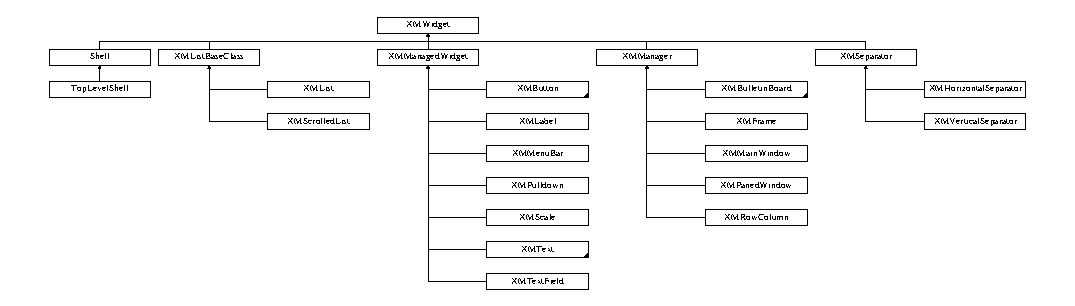
\includegraphics[height=3.66013cm]{classXMWidget}
\end{center}
\end{figure}
\subsection*{Public Methods}
\begin{CompactItemize}
\item 
{\bf XMWidget} (char $\ast$n)
\item 
{\bf XMWidget} (Widget w)
\item 
{\bf XMWidget} (char $\ast$n, Widget\-Class cl, {\bf XMApplication} \&parent, Arg\-List l=NULL, Cardinal num\_\-args=0)
\item 
{\bf XMWidget} (char $\ast$n, Widget\-Class cl, Widget parent, Arg\-List l=NULL, Cardinal num\_\-args=0)
\item 
{\bf XMWidget} (char $\ast$n, Widget\-Class cl, XMWidget \&parent, Arg\-List l=NULL, Cardinal num\_\-args=0)
\item 
virtual {\bf $\sim$XMWidget} ()
\item 
Widget {\bf getid} ()
\item 
Widget {\bf getparent} ()
\item 
char $\ast$ {\bf getname} ()
\item 
void {\bf Set\-Attribute} (String attribute, Xt\-Arg\-Val value)
\item 
void {\bf Set\-Attribute} (String attribute, void $\ast$value)
\item 
void {\bf Get\-Attribute} (String attribute, void $\ast$value)
\item 
void {\bf Get\-Attribute} (String attribute, Xt\-Arg\-Val value)
\item 
{\bf Callback\_\-data} $\ast$ {\bf Add\-Callback} (String reason, void($\ast$proc)(XMWidget $\ast$, Xt\-Pointer, Xt\-Pointer), Xt\-Pointer data=NULL)
\item 
void {\bf Map} ()
\item 
void {\bf Un\-Map} ()
\item 
void {\bf Manage} ()
\item 
void {\bf Un\-Manage} ()
\item 
void {\bf Realize} ()
\item 
void {\bf Un\-Realize} ()
\end{CompactItemize}
\subsection*{Protected Methods}
\begin{CompactItemize}
\item 
void {\bf Create} (char $\ast$n, Widget\-Class cl, Widget parent, Arg\-List l, Cardinal num\_\-args)
\end{CompactItemize}
\subsection*{Protected Attributes}
\begin{CompactItemize}
\item 
Widget {\bf id}
\item 
{\bf XMWidget\-Name} {\bf name}
\end{CompactItemize}


\subsection{Constructor \& Destructor Documentation}
\index{XMWidget@{XMWidget}!XMWidget@{XMWidget}}
\index{XMWidget@{XMWidget}!XMWidget@{XMWidget}}
\subsubsection{\setlength{\rightskip}{0pt plus 5cm}XMWidget::XMWidget (char $\ast$ {\em n})\hspace{0.3cm}{\tt  [inline]}}\label{classXMWidget_a0}




Definition at line 375 of file XMWidget.h.

References name.\index{XMWidget@{XMWidget}!XMWidget@{XMWidget}}
\index{XMWidget@{XMWidget}!XMWidget@{XMWidget}}
\subsubsection{\setlength{\rightskip}{0pt plus 5cm}XMWidget::XMWidget (Widget {\em w})\hspace{0.3cm}{\tt  [inline]}}\label{classXMWidget_a1}




Definition at line 380 of file XMWidget.h.

References id, and name.\index{XMWidget@{XMWidget}!XMWidget@{XMWidget}}
\index{XMWidget@{XMWidget}!XMWidget@{XMWidget}}
\subsubsection{\setlength{\rightskip}{0pt plus 5cm}XMWidget::XMWidget (char $\ast$ {\em n}, Widget\-Class {\em cl}, {\bf XMApplication} \& {\em parent}, Arg\-List {\em l} = NULL, Cardinal {\em num\_\-args} = 0)\hspace{0.3cm}{\tt  [inline]}}\label{classXMWidget_a2}




Definition at line 385 of file XMWidget.h.

References Create(), and XMApplication::getid().\index{XMWidget@{XMWidget}!XMWidget@{XMWidget}}
\index{XMWidget@{XMWidget}!XMWidget@{XMWidget}}
\subsubsection{\setlength{\rightskip}{0pt plus 5cm}XMWidget::XMWidget (char $\ast$ {\em n}, Widget\-Class {\em cl}, Widget {\em parent}, Arg\-List {\em l} = NULL, Cardinal {\em num\_\-args} = 0)\hspace{0.3cm}{\tt  [inline]}}\label{classXMWidget_a3}




Definition at line 390 of file XMWidget.h.

References Create().\index{XMWidget@{XMWidget}!XMWidget@{XMWidget}}
\index{XMWidget@{XMWidget}!XMWidget@{XMWidget}}
\subsubsection{\setlength{\rightskip}{0pt plus 5cm}XMWidget::XMWidget (char $\ast$ {\em n}, Widget\-Class {\em cl}, XMWidget \& {\em parent}, Arg\-List {\em l} = NULL, Cardinal {\em num\_\-args} = 0)\hspace{0.3cm}{\tt  [inline]}}\label{classXMWidget_a4}




Definition at line 395 of file XMWidget.h.

References Create(), and getid().\index{XMWidget@{XMWidget}!~XMWidget@{$\sim$XMWidget}}
\index{~XMWidget@{$\sim$XMWidget}!XMWidget@{XMWidget}}
\subsubsection{\setlength{\rightskip}{0pt plus 5cm}virtual XMWidget::$\sim$XMWidget ()\hspace{0.3cm}{\tt  [inline, virtual]}}\label{classXMWidget_a5}




Definition at line 400 of file XMWidget.h.

References id.

\subsection{Member Function Documentation}
\index{XMWidget@{XMWidget}!AddCallback@{AddCallback}}
\index{AddCallback@{AddCallback}!XMWidget@{XMWidget}}
\subsubsection{\setlength{\rightskip}{0pt plus 5cm}{\bf Callback\_\-data}$\ast$ XMWidget::Add\-Callback (String {\em reason}, void($\ast$ {\em proc})(XMWidget $\ast$, Xt\-Pointer, Xt\-Pointer), Xt\-Pointer {\em data} = NULL)\hspace{0.3cm}{\tt  [inline]}}\label{classXMWidget_a13}




Definition at line 419 of file XMWidget.h.

References XMAdd\-Callback().

Referenced by XMText\-Field::Add\-Activate\-Callback(), XMList\-Base\-Class::Addbrowse\-Selection\-Callback(), XMArrow\-Button::Add\-Callback(), XMToggle\-Button::Add\-Callback(), XMCascade\-Button::Add\-Callback(), XMPush\-Button::Add\-Callback(), XMScale::Add\-Changed\-Callback(), XMList\-Base\-Class::Add\-Default\-Action\-Callback(), XMScale::Add\-Drag\-Callback(), XMRow\-Column::Add\-Entry\-Callback(), XMList\-Base\-Class::Add\-Extended\-Selection\-Callback(), XMManager::Add\-Help\-Callback(), XMList\-Base\-Class::Add\-Multiple\-Selection\-Callback(), XMList\-Base\-Class::Add\-Single\-Selection\-Callback(), XMArrow\-Button::XMArrow\-Button(), XMCascade\-Button::XMCascade\-Button(), XMPush\-Button::XMPush\-Button(), and XMToggle\-Button::XMToggle\-Button().\index{XMWidget@{XMWidget}!Create@{Create}}
\index{Create@{Create}!XMWidget@{XMWidget}}
\subsubsection{\setlength{\rightskip}{0pt plus 5cm}void XMWidget::Create (char $\ast$ {\em n}, Widget\-Class {\em cl}, Widget {\em parent}, Arg\-List {\em l}, Cardinal {\em num\_\-args})\hspace{0.3cm}{\tt  [inline, protected]}}\label{classXMWidget_b0}




Definition at line 366 of file XMWidget.h.

References id, and name.

Referenced by XMWidget().\index{XMWidget@{XMWidget}!GetAttribute@{GetAttribute}}
\index{GetAttribute@{GetAttribute}!XMWidget@{XMWidget}}
\subsubsection{\setlength{\rightskip}{0pt plus 5cm}void XMWidget::Get\-Attribute (String {\em attribute}, Xt\-Arg\-Val {\em value})\hspace{0.3cm}{\tt  [inline]}}\label{classXMWidget_a12}




Definition at line 416 of file XMWidget.h.

References id.\index{XMWidget@{XMWidget}!GetAttribute@{GetAttribute}}
\index{GetAttribute@{GetAttribute}!XMWidget@{XMWidget}}
\subsubsection{\setlength{\rightskip}{0pt plus 5cm}void XMWidget::Get\-Attribute (String {\em attribute}, void $\ast$ {\em value})\hspace{0.3cm}{\tt  [inline]}}\label{classXMWidget_a11}




Definition at line 414 of file XMWidget.h.

References id.

Referenced by XMArrow\-Button::Direction(), Shell::Get\-Geometry(), Top\-Level\-Shell::Get\-Iconic(), Top\-Level\-Shell::Get\-Icon\-Name(), XMList\-Base\-Class::Get\-List\-Count(), XMList\-Base\-Class::Get\-List\-Values(), Shell::Get\-Save\-Under(), XMList\-Base\-Class::Get\-Selected\-Items(), XMList\-Base\-Class::Get\-Selected\-List\-Count(), XMToggle\-Button::Get\-State(), and Shell::Is\-Resize\-Allowed().\index{XMWidget@{XMWidget}!getid@{getid}}
\index{getid@{getid}!XMWidget@{XMWidget}}
\subsubsection{\setlength{\rightskip}{0pt plus 5cm}Widget XMWidget::getid ()\hspace{0.3cm}{\tt  [inline]}}\label{classXMWidget_a6}




Definition at line 404 of file XMWidget.h.

References id.

Referenced by XMMenu\-Bar::Add\-Help\-Pulldown(), XMCallback$<$ Shell $>$::Register(), XMMain\-Window::Set\-Areas(), XMCascade\-Button::Set\-Associated\-Menu(), XMForm::Set\-Bottom\-Widget(), XMForm::Set\-Left\-Widget(), XMForm::Set\-Right\-Widget(), XMForm::Set\-Top\-Widget(), Shell::Shell(), XMCallback$<$ Shell $>$::Un\-Register(), XM\_\-help(), XMAdd\-Callback(), XMForm::XMForm(), XMMenu\-Bar::XMMenu\-Bar(), XMPulldown::XMPulldown(), XMRemove\-Callback(), XMScrolled\-List::XMScrolled\-List(), XMScrolled\-Text::XMScrolled\-Text(), and XMWidget().\index{XMWidget@{XMWidget}!getname@{getname}}
\index{getname@{getname}!XMWidget@{XMWidget}}
\subsubsection{\setlength{\rightskip}{0pt plus 5cm}char$\ast$ XMWidget::getname ()\hspace{0.3cm}{\tt  [inline]}}\label{classXMWidget_a8}




Definition at line 406 of file XMWidget.h.

References name.

Referenced by XMPulldown::Find\-Menu\-Item(), and XMMenu\-Bar::Get\-Pulldown().\index{XMWidget@{XMWidget}!getparent@{getparent}}
\index{getparent@{getparent}!XMWidget@{XMWidget}}
\subsubsection{\setlength{\rightskip}{0pt plus 5cm}Widget XMWidget::getparent ()\hspace{0.3cm}{\tt  [inline]}}\label{classXMWidget_a7}




Definition at line 405 of file XMWidget.h.

References id.\index{XMWidget@{XMWidget}!Manage@{Manage}}
\index{Manage@{Manage}!XMWidget@{XMWidget}}
\subsubsection{\setlength{\rightskip}{0pt plus 5cm}void XMWidget::Manage ()\hspace{0.3cm}{\tt  [inline]}}\label{classXMWidget_a16}




Reimplemented in {\bf XMScrolled\-List} {\rm (p.\,\pageref{classXMScrolledList_a3})}, and {\bf Shell} {\rm (p.\,\pageref{classShell_a9})}.

Definition at line 433 of file XMWidget.h.

References id.

Referenced by XMHorizontal\-Separator::XMHorizontal\-Separator(), XMList::XMList(), XMManaged\-Widget::XMManaged\-Widget(), and XMVertical\-Separator::XMVertical\-Separator().\index{XMWidget@{XMWidget}!Map@{Map}}
\index{Map@{Map}!XMWidget@{XMWidget}}
\subsubsection{\setlength{\rightskip}{0pt plus 5cm}void XMWidget::Map ()\hspace{0.3cm}{\tt  [inline]}}\label{classXMWidget_a14}




Definition at line 431 of file XMWidget.h.

References id.\index{XMWidget@{XMWidget}!Realize@{Realize}}
\index{Realize@{Realize}!XMWidget@{XMWidget}}
\subsubsection{\setlength{\rightskip}{0pt plus 5cm}void XMWidget::Realize ()\hspace{0.3cm}{\tt  [inline]}}\label{classXMWidget_a18}




Reimplemented in {\bf Shell} {\rm (p.\,\pageref{classShell_a8})}.

Definition at line 435 of file XMWidget.h.

References id.\index{XMWidget@{XMWidget}!SetAttribute@{SetAttribute}}
\index{SetAttribute@{SetAttribute}!XMWidget@{XMWidget}}
\subsubsection{\setlength{\rightskip}{0pt plus 5cm}void XMWidget::Set\-Attribute (String {\em attribute}, void $\ast$ {\em value})\hspace{0.3cm}{\tt  [inline]}}\label{classXMWidget_a10}




Definition at line 411 of file XMWidget.h.

References id.\index{XMWidget@{XMWidget}!SetAttribute@{SetAttribute}}
\index{SetAttribute@{SetAttribute}!XMWidget@{XMWidget}}
\subsubsection{\setlength{\rightskip}{0pt plus 5cm}void XMWidget::Set\-Attribute (String {\em attribute}, Xt\-Arg\-Val {\em value})\hspace{0.3cm}{\tt  [inline]}}\label{classXMWidget_a9}




Definition at line 409 of file XMWidget.h.

References id.

Referenced by XMMenu\-Bar::Add\-Help\-Pulldown(), XMPulldown::Add\-Menu\-Button(), XMPulldown::Add\-Menu\-Toggle\-Button(), XMRow\-Column::Align(), XMBulletin\-Board::Allow\-Overlap(), Shell::Allow\-Resize(), XMPaned\-Window::Allow\-Resize(), XMList\-Base\-Class::Auto\-Select(), XMToggle\-Button::Box(), XMMain\-Window::Command\-Window\-Location(), XMToggle\-Button::Diamond(), XMButton::Disable(), XMText::Disable\-Word\-Wrap(), XMButton::Enable(), XMText\-Field::Enable\-Word\-Wrap(), XMText::Enable\-Word\-Wrap(), XMToggle\-Button::Hide\-Indicator(), XMButton::Label(), XMPaned\-Window::Margins(), XMRow\-Column::Margins(), XMFrame::Margins(), XMBulletin\-Board::Margins(), XMPaned\-Window::Max\-Pane\-Size(), XMPaned\-Window::Min\-Pane\-Size(), XMPulldown::No\-Radio\-Menu(), XMRow\-Column::No\-Radio\-Menu(), XMArrow\-Button::Point\-Down(), XMArrow\-Button::Point\-Left(), XMArrow\-Button::Point\-Right(), XMArrow\-Button::Point\-Up(), XMPulldown::Radio\-Force\-One(), XMRow\-Column::Radio\-Force\-One(), XMPulldown::Radio\-Menu(), XMRow\-Column::Radio\-Menu(), XMPulldown::Radio\-No\-Force\-One(), XMRow\-Column::Radio\-No\-Force\-One(), Top\-Level\-Shell::Realize\-Iconic(), XMToggle\-Button::Set(), XMRow\-Column::Set\-Alignment(), XMMain\-Window::Set\-Areas(), XMCascade\-Button::Set\-Associated\-Menu(), XMWidget\-List::Set\-Attribute(), XMText\-Field::Set\-Columns(), XMText::Set\-Columns(), XMManager::Set\-Constraint(), XMList\-Base\-Class::Set\-Double\-Click\-Time(), XMText::Set\-Editing(), XMRow\-Column::Set\-Entry\-Class(), XMForm::Set\-Fraction\-Base(), Shell::Set\-Geometry(), XMRow\-Column::Set\-Homogenous(), XMForm::Set\-Horizontal\-Spacing(), Top\-Level\-Shell::Set\-Icon\-Name(), XMLabel::Set\-Label(), XMText\-Field::Set\-Max\-Length(), XMText::Set\-Max\-Length(), XMButton::Set\-Mnemonic(), XMManager::Set\-Navigation\-Type(), XMSeparator::Set\-Orientation(), XMRow\-Column::Set\-Orientation(), XMRow\-Column::Set\-Packing(), XMPaned\-Window::Set\-Pane\-Spacing(), XMRow\-Column::Set\-Row\-Columns(), XMText::Set\-Rows(), XMList\-Base\-Class::Set\-Rows(), XMForm::Set\-Rubber\-Positioning(), XMPaned\-Window::Set\-Sash\-Height(), XMPaned\-Window::Set\-Sash\-Indent(), Shell::Set\-Save\-Under(), XMList\-Base\-Class::Set\-Scroll\-Policy(), XMList\-Base\-Class::Set\-Selection\-Policy(), XMPaned\-Window::Set\-Separator(), XMSeparator::Set\-Shadow\-Type(), XMFrame::Set\-Shadow\-Type(), XMBulletin\-Board::Set\-Shadow\-Type(), XMRow\-Column::Set\-Spacing(), XMToggle\-Button::Set\-State(), XMForm::Set\-Vertical\-Spacing(), XMToggle\-Button::Show\-Indicator(), XMMain\-Window::Show\-Separator(), XMPaned\-Window::Skip\-Adjust(), XMManager::Traversal\-On(), XMManager::Traverse\-Off(), and XMToggle\-Button::Un\-Set().\index{XMWidget@{XMWidget}!UnManage@{UnManage}}
\index{UnManage@{UnManage}!XMWidget@{XMWidget}}
\subsubsection{\setlength{\rightskip}{0pt plus 5cm}void XMWidget::Un\-Manage ()\hspace{0.3cm}{\tt  [inline]}}\label{classXMWidget_a17}




Reimplemented in {\bf XMScrolled\-List} {\rm (p.\,\pageref{classXMScrolledList_a4})}, and {\bf Shell} {\rm (p.\,\pageref{classShell_a10})}.

Definition at line 434 of file XMWidget.h.

References id.

Referenced by XMUnmanage\-Child().\index{XMWidget@{XMWidget}!UnMap@{UnMap}}
\index{UnMap@{UnMap}!XMWidget@{XMWidget}}
\subsubsection{\setlength{\rightskip}{0pt plus 5cm}void XMWidget::Un\-Map ()\hspace{0.3cm}{\tt  [inline]}}\label{classXMWidget_a15}




Definition at line 432 of file XMWidget.h.

References id.\index{XMWidget@{XMWidget}!UnRealize@{UnRealize}}
\index{UnRealize@{UnRealize}!XMWidget@{XMWidget}}
\subsubsection{\setlength{\rightskip}{0pt plus 5cm}void XMWidget::Un\-Realize ()\hspace{0.3cm}{\tt  [inline]}}\label{classXMWidget_a19}




Definition at line 436 of file XMWidget.h.

References id.

\subsection{Member Data Documentation}
\index{XMWidget@{XMWidget}!id@{id}}
\index{id@{id}!XMWidget@{XMWidget}}
\subsubsection{\setlength{\rightskip}{0pt plus 5cm}Widget XMWidget::id\hspace{0.3cm}{\tt  [protected]}}\label{classXMWidget_n0}




Definition at line 364 of file XMWidget.h.

Referenced by XMList\-Base\-Class::Add\-Item(), XMScrolled\-Text::Add\-Text(), XMPulldown::Build\-Menu(), XMList\-Base\-Class::Clear\-Items(), XMScrolled\-Text::Clear\-Text(), Create(), XMList\-Base\-Class::Delete\-Item(), XMList\-Base\-Class::Delete\-Items(), XMList\-Base\-Class::Deselect\-All(), XMList\-Base\-Class::Deselect\-Item(), Get\-Attribute(), getid(), getparent(), XMText\-Field::Get\-Text(), XMText::Get\-Text(), Manage(), Shell::Manage(), XMScrolled\-List::Manage(), Map(), XMMenu\-Bar::mb\-Create(), Realize(), Shell::Realize(), XMList\-Base\-Class::Select\-Item(), XMButton::Set\-Accelerator(), Set\-Attribute(), XMList\-Base\-Class::Set\-Bottom\-Item(), XMScale::Set\-Range(), XMText\-Field::Set\-Text(), XMText::Set\-Text(), Shell::Shell(), Un\-Manage(), Shell::Un\-Manage(), XMScrolled\-List::Un\-Manage(), Un\-Map(), Un\-Realize(), XMScale::Value(), XMForm::XMForm(), XMFrame::XMFrame(), XMMain\-Window::XMMain\-Window(), XMPaned\-Window::XMPaned\-Window(), XMRow\-Column::XMRow\-Column(), XMScrolled\-List::XMScrolled\-List(), XMScrolled\-Text::XMScrolled\-Text(), XMWidget(), and $\sim$XMWidget().\index{XMWidget@{XMWidget}!name@{name}}
\index{name@{name}!XMWidget@{XMWidget}}
\subsubsection{\setlength{\rightskip}{0pt plus 5cm}{\bf XMWidget\-Name} XMWidget::name\hspace{0.3cm}{\tt  [protected]}}\label{classXMWidget_n1}




Definition at line 365 of file XMWidget.h.

Referenced by XMPulldown::Add\-Menu\-Button(), XMPulldown::Add\-Menu\-Toggle\-Button(), XMPulldown::Build\-Menu(), Create(), Top\-Level\-Shell::Get\-Icon\-Name(), getname(), XMMenu\-Bar::mb\-Create(), Top\-Level\-Shell::Set\-Icon\-Name(), XMForm::XMForm(), XMFrame::XMFrame(), XMMain\-Window::XMMain\-Window(), XMPaned\-Window::XMPaned\-Window(), XMRow\-Column::XMRow\-Column(), and XMWidget().

The documentation for this class was generated from the following file:\begin{CompactItemize}
\item 
{\bf XMWidget.h}\end{CompactItemize}
